\documentclass[12pt,english]{scrartcl}

\usepackage{amsmath,amssymb}
%\usepackage[amssymb]{SIunits}
\usepackage{babel}
\usepackage[latin1]{inputenc}
\usepackage{graphicx}
\usepackage{color}
\usepackage{url}


\begin{document}

\begin{center}
\textbf{\begin{LARGE}KOGW-PM-KNP:\\ \vspace{3mm} Tutorial 11 - The El Greco Fallacy in Perception Research
\end{LARGE}}
\end{center}

This tutorial deals with a particular kind of cognitive bias. The paper by Firestone \& Scholl (2016) introduces a certain kind of bias and suggests that the rationale of several paradigms in perception research are contaminated by that very bias. Please read the paper critically. Answer the following questions which should help you to evaluate their findings. Please work in pairs. 
%  
% \begin{figure}[htbp]
% \begin{center}
% 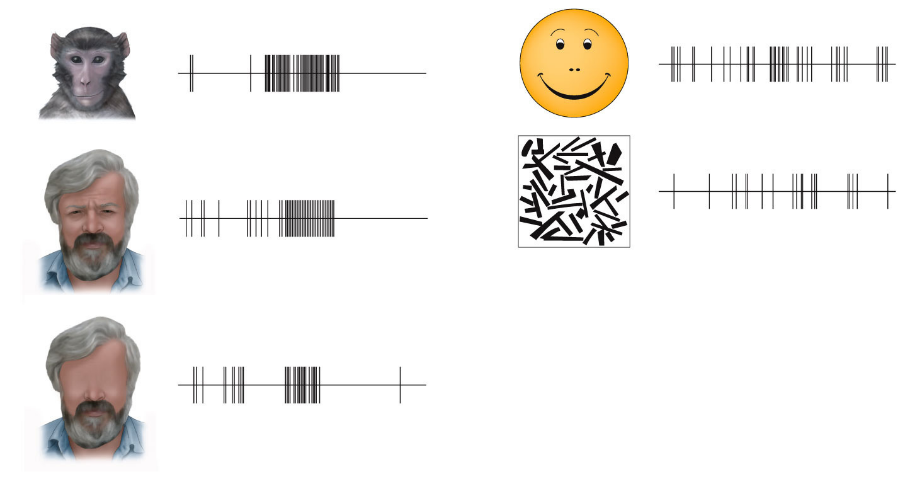
\includegraphics[width = 0.8\textwidth]{IT_cell.png}
% \end{center}
% \caption{
% \label{fig:IT_cell}}
% \end{figure}

\begin{enumerate}
 \item What does the \textit{cognitively impenetrability} hypothesis of perception say? Name one type of evidence that supports the hypothesis.

 \item Explain the El Greco Fallacy with the help of a sketch that illustrates stimuli in the outside world, how they are perceived and how they would be painted.


 \item Describe the original finding that the authors wanted to replicate in their Experiment 1.

 \item Describe the procedure and results of experiment 1.


 \item Describe the procedure and logic underlying experiment 2. What were the results?
 
 \item What type of effect do the experimenters test in Experiment 3? Describe the procedure and the results.

\item What do the authors suggest as a reason for why it has been difficult to provide evidence for the absence of top-down effects. 
 

\item Do you perceive any problems with the research reported in the article - with respect to methodology, reasoning, ... etc.? 
\end{enumerate}

\end{document}
